\chapter{Design} % ~ 10+ pages
\label{chap:design}
% Theoretical Basis for Implementation
    % What am I doing and why?
The research for this thesis is mainly performed with the help of brain simulations. Therefore this chapter first supplies an overview of the simulation environment and how the simulations were performed. Followed by a detailed discussion of design choices regarding the simulation input, the output analysis, and the electromagnetic attack. The focus is set on drawing connections to the theoretical basis that was laid out in the previous chapter.

\section{Research Scenario}
% Research setup
Before more specific work of this thesis is elaborated on, this section presents the environment, in which the research was performed. This first and foremost includes a description of the simulator, and how it was used to run simulations of the hippocampus. But also the model of the hippocampus shall be explained with its most important parameters, as well as the needed input and resulting output values.

    \subsection{Simulation Model} % Compare old with new model code (mention differences)?
    % Elaborations on brian2
        % library for Python that allows to create and run models for spiking neural networks
        % Its simulations work with the help of mathematical abstractions for neurons
    Brian2 was used to run all the simulations presented in this thesis. This simulator was created as a Python library and allows simulations of spiking neural networks to be run. It works with mathematical abstractions of neurons and synapses, instead of creating anatomically accurate structures, which reduces the computational load and therefore increases simulation speed and efficiency \cite{Brian2}. \\
    % elaborate on aspects of the model, that are needed to understand my approach and output
        % stay high level enough
    % small to big structures, that are being represented in the model
        % neurons = collection of equations
        % can be connected with each other and large networks formed
        % This model makes use of different neuron models to represent what exist in brain
        % spatially accurate organized
        % Comparision image brain - 2d network structure / or only 3d image
    With Brain2 it is possible to create rather large simulation models (of many neurons and synapses), without requiring a supercomputer to run them. This is something that the employed model of the hippocampus also profits from, as it (in its standard configuration) contains the abstractions of over 30'000 model neurons. In accordance with the anatomy of the hippocampus, this includes different types of neurons. Each of them being defined by a collection of equations and values, which reflect their real properties in a mathematical form. For example the conductance of ion channels that they possess \cite{Aussel.2018}.
    
    This model distributes these neurons in space, such that an anatomically accurate, 15mm thick slice of the hippocampus and entorhinal cortex is created. Respecting also the ratio of each neuron type in different structures and areas (see Figure \ref{fig:hippocampus-model}). Connections between the neurons are then also formed in accordance with the existing literature. Promoting known signal pathways and respecting the factor of distance. From a technical standpoint, this has been realized by defining the probabilities for synaptic connections between neurons accordingly \cite{Aussel.2018}.\\
    Essentially all these neuron and synapse-related parameters can be adjusted to explore their effect on the network activity. But especially in the newer version of the model code \cite{HippSimModel.2} (which was released with the following paper \cite{Aussel.2022} in 2022), it is possible to easily adjust many further and more general aspects of the model. This includes for example the option to choose between waking or sleeping connectivity settings or to change the level of a neurotransmitter. By selecting proper values for this large parameter space, it is possible to recreate many different states of the brain and observe how the network activity changes. 
    
        
    \subsection{Simulation Process}
    % ?create diagram for process flow?
    % How does a generic simulation of it work
        % Input via EC (mention necessity of creating stereotypical input)
        % time frame wise simulation/calculation of electric activity
        % Output (LFP measurements) - mention briefly why that relevant and what can be analysed/ how interpreted
            % example image?
    When the parameters of the network are configured, its activity may be observed by running a simulation. This will in a first step, trigger the generation of the network with the defined parameters.\\
    As soon as everything is set up, the \textbf{input} will be injected into the network. This input represents the stimulation of the hippocampus by the other areas of the brain. Since this external stimulation reaches the hippocampus mostly via the EC, the model only applies the input stimulation to the neurons of this structure. From there the signals are then propagated to the other areas \cite{Aussel.2018}. Multiple types of inputs can be supplied to the model. A realistic approach is to recreate the activity of a real EC with the help of EEG recordings. But also stereotypical inputs may or have to be used when such files are not available.\\
    The \textbf{activity} of each neuron is then simulated during time frames of 100ms. After each of these time frames, the electrical potential inside the network is calculated and recorded \cite{HippSimModel.1}. The main recording is performed along a cylinder of 0.8 mm diameter, which is the size of an electrode that would be used in real brain recordings. This ensures, that the simulation produces an output that is comparable to in vivo recordings \cite{Aussel.2018}.\\
    The \textbf{output} values that are collected like this, are local field potentials (LFP). They represent the extracellular electrical potential in the area of the simulated electrode and therefore provide information about the accumulated activity of many neurons \cite{Aussel.2018}. Followingly, the output can be used well to identify activity patterns of larger neuron populations, which is precisely what is necessary for this work. 
    
    
    \subsection{Model Adjustments and Configuration}
    % Elaborate on most important changes that were necessary to get it running/optimize performance
        % what my standard running configuration was (high level)
            % Mention setup with different input/connectivity combinations
            % explain why only (wake)/sleep relevant/realistic
    % Computer resources used for the simulations
    As mentioned before, there exist two different versions of the model code. One was released in 2018 \cite{HippSimModel.1}, following the paper of \textcite{Aussel.2018}, where it was used to investigate the sleep-wake cycle and related activity patterns. The second version was then released in 2022 \cite{HippSimModel.2}, accompanying another paper of \textcite{Aussel.2022}, concerned with exploring mechanisms involved in epilepsy.\\
    Since the original use case of the \textbf{first model} was most similar to the one in this thesis, it was used for the initial simulation work. Unfortunately, both versions of the model code do not contain the EEG files that were used as input in the related papers. Therefore, it was necessary to develop an alternative input, to be able to run the simulation. But before the development and optimization of this input, was possible in a reasonable time frame, it was necessary to perform some debugging and configuration adjustments. This incorporated mostly code adjustments, to parameterize the running configuration, such that only relevant scenarios were executed. Effectively reducing the simulation time by a factor of 4, which still amounted to about 10 hours of processing per 60 seconds of simulated activity. Details regarding the input design, its implementation, and evaluation, will be presented in the according chapters.\\
    Just as this process concluded, the model creator was able to supply input EEG files, allowing for even more realistic simulations. Further, it was revealed that the \textbf{second version} of the model only was an improved version, with additional functionality related to epilepsy simulations. Still including the functionality of the primary model, whilst also improving the code quality and parameterization. Therefore, all the following work was performed in this version, utilizing the EEG files as input. Even though this rendered some work on the first model obsolete, the most relevant parts could easily be transferred to this newer version. Ultimately allowing for an optimized and more realistic simulation environment for the investigation of electromagnetic attacks and their underlying mechanisms. 

    % Evaluation of memory performance is the goal
        % -> healthy sleeping configuration serves as the base case
            % because swrs pretty much restricted to it
        % -> Adjustments of the parameters shall reflect the impact of an electromagnetic attack
    The model in general allows for the simulation of many parameter configurations, of which not all were relevant for the work of this thesis. Since the general goal is to evaluate the performance of memory consolidation, the sleeping state and its activity under healthy conditions were considered the base case. This choice was made because most of the activity that is related to memory consolidation takes place during sleep \cite{BUZSAKI1989551}. Adjustments to this base configuration were then performed to reflect for example the impact of an electromagnetic attack.\\
    % computer setup (develop on win, run on vm-linux), and resulting runtime of simulations
    Whilst the development of the code and output analysis was performed on a Windows computer, the simulations were executed on a Linux virtual machine, supplied by the Communication Systems Research Group (CSG) at the Department of Informatics (IfI) of the University of Zurich (UZH). Utilizing a CPU with 8 cores, running at 2.4GHz each, led to an average simulation time of approximately 10 hours (employing the second model version and performing 8 simulations of 60s simultaneously). 

\section{Simulation Input}
% Inputs are a necessary parameter for simulations
% generally two options: realistic eeg files, stereotypical one
    % none available in the first model code
        % suitable eeg files difficult to attain
        % had to design my own stereotypical (even though eeg files would have been preferable)
    % Then received EEG files
        % better / more relevant than stereotypical input
            % made old one obsolete (for attack simulations only EEG files)
    % But development of stereotypical input yielded interesting findings anyway
        % about impact of input on relevant output
        % allows for comparison between both (in evaluation)
% In the following, specifics about the two types of inputs used and how they are integrated into the sim (on a theoretical basis)
As mentioned above, the simulation input is a necessary parameter, to simulate relevant activity in the model \cite{Aussel.2021}. There are generally two possible ways to supply an input. Either, with the help of EEG files (constituting real measurements of brain activity) or by synthetically creating one. In the process of this work, both input types were explored and used for simulations. Even though the more realistic option of utilizing EEG files was preferred for the rest of the work, the design of the synthetic input offered some relevant insight nonetheless. More details on that regard as well as a comparison between the two, can be found in the evaluation chapter. In the following, specifics about their design choices will be presented. 

    \subsection{Synthetic Input}
    % based on the input equation of the paper
        % relevance
            % can reproduce activity patterns
        % Explain main parameters of adjustment
            % amplitude and Frequency
    % present further input reference I used for the design
        % outputs from model paper that lead to the decision of integration of further params in input equation
            % LFP readings and general shape/occurrence of activity spikes
                % explain wave realization param
        % other outputs i then (tried to) reproduce
    The design of the synthetic input was based on the work of \textcite{Aussel.2021}, which followed the paper associated with the first model \cite{Aussel.2018}. In the context of a large parameter analysis of the model, they propose a stereotypical alternative input, to their EEG files. This input comprises a square wave current \(I_{\text{stim}}\), which is injected into all neurons of the entorhinal cortex and is defined by the following equation:
    %
    \[I_{\text{stim}}(t) = 
    \begin{cases} 
    A_1 & \text{if } \{ t > t_0 \text{ and } \sin(2\pi f_1 (t - t_0)) \geq 0 \} \\ 
    0 & \text{otherwise} 
    \end{cases}\]
    \\
    Whilst \(t\) represents the current simulation time, \(t_0\) defines the starting time of the input (with a recommended value of \(250ms\)). The core parameters for adjustments are then the remaining variables \(A_1\) standing for the \textit{amplitude} and \(f_1\) representing the \textit{frequency} of the generated input wave \cite{Aussel.2021}.

    To recreate a similar model behavior as \textcite{Aussel.2018} produced with the help of EEG files, a closer analysis of their documented output, and especially sleep LFP traces was performed. This led to the observation of relatively long breaks between short activity phases in their signal, which motivated the integration of another parameter into the equation. Specifically \(w\), which defines the interval of realized waves. Adding the possibility to also expand the time in between stimulation waves, without changing the \textit{frequency} and therefore the length of a stimulating wave. The adjusted equation looks like this: 
    %
    \[I_{\text{stim}}(t) = 
    \begin{cases} 
    A_1 & \text{if } t \geq t_0 \text{ and } \sin(2\pi f_1 (t - t_0)) \geq 0 \text{ and } \left( \left\lfloor \frac{t - t_0}{T} \right\rfloor \mod w = 0 \right) \\ 
    0 & \text{otherwise} 
    \end{cases}\]
    %
    Where \(T\) stands for the time of a wave period and is defined as \(\frac{1}{f_1}\). How the output of the model varied, depending on these parameters and which combination yielded the best results is the subject of the evaluation chapter. However, a general range of relevant and realistic parameter values was already identified by \textcite{Aussel.2021}. Restricting the exploration to values of \(A_1 : [0.5nA, 1.5nA]\) and \(f_1 : [0Hz, 10Hz]\).

    
    \subsection{Realistic Input}
    % elaborate on late reception of files
        % model creator was able to supply
        % recently received permission from data "owners" to pass on for scientific (against the previous statement)
    % elaborate on EEG files as input
        % how they were created/preprocessed
        % how integrated in sim, in comparison to stereotypical
        % expected benefits from realistic input
    Contrary to what the model creator stated in the context of the code release, it was possible to get access to EEG files that were used in \cite{Aussel.2022}. These files are the result of recordings that were made with the help of stereoelectroencephalography (SEEG) \cite{Aussel.2018}, which is an invasive form of EEG \cite{Minotti.2018}. With a sampling frequency of 1024 Hz, they were collected from brain areas connected to the hippocampus, in subjects suffering from epilepsy. With the help of a neurologist, they were categorized as sleep and wake recording, and epileptic activity was identified. Resulting in files representing healthy or epileptic activity during sleep or waking state \cite{Aussel.2018}. This work generally utilized the files representing healthy activity during the sleeping state, as input.

    The integration of these files into the simulation is performed with the help of three neuron groups, that represent the brain areas of the recorded activity. Each group is connected to a different slice of the entorhinal cortex, via excitatory synapses that are formed with a uniform probability. The activity of these neuron groups is defined by transforming the measurements of the input files into firing rates, by scaling them to a maximum value of 200Hz. Because each group's activity is based on a different file, recorded from a different area, their activity differs. However, the activity of each neuron inside a group is the same \cite{Aussel.2022} \cite{HippSimModel.1}.
    
    

\section{Simulation Output Analysis}
% Recap, Sim produces LFP readings as output
    % Representing electrical activity of a larger group of neurons
    % giving idea about general activity of hippocampal formation
% For work relevant is performance of long-term memory consolidation
    % associated with a specific activity pattern in hipp
        % Sharp Wave ripples (ref)
    % need to analyze the output values for the pattern
        % exist different approaches
        % no consensus on correct way
% (section structure:) first elaborating on SWR, then presenting two detection approaches
The main output of a simulation with the model is a text file containing local field potentials. These values imitate recordings that would arise if an electrode were placed inside the simulated network. To achieve this, the model calculates the extracellular electrical potential of the neurons in a certain area with a sampling frequency of 1024Hz (resulting in 1024 values per simulated second) \cite{HippSimModel.2}.\\
Even though these recordings already can supply an impression of the general network activity when plotted, further analysis is necessary to investigate more specific behaviors of the model. As this work tries to evaluate the performance of memory consolidation in different brain states, the analysis needs to yield a measure for that. What has been identified as such a measure, is the occurrence of sharp wave ripples (SWRs).\\
In the following section, SWRs and their properties are discussed, before the detection approach is explored.

        
    \subsection{Sharp Wave Ripples}
    % Detectable in network scale activity
    % from large groups of neurons, not single ones
        % LFP well-suited
    % How are they characterized in LFP traces
        % Composition of
            % Sharp Wave
                % strong signal
                % many neurons fire extremely synchronized
            % Ripple
                % Defines Oscillation frequency band
                % LFP fluctuations
    % show plot(s)
    Sharp wave ripples (or sharp wave ripple complexes) represent a synchronized activity pattern, of neuron populations \cite{Buzsaki.2015}, which allows for their detection based on LFP recordings \cite{Liu.2022}. They play a critical role in memory consolidation \cite{Girardeau.2011} \cite{AmelieAussel.2020}, which is why they were chosen as a measure of its performance. They are characterized by the coupling of two events, specifically a \textit{sharp wave} and a \textit{ripple} \cite{Buzsaki.2015}.\\
    The \textbf{sharp wave} represents a deflection in the LFP signal of large amplitude. Usually lasting for about 40-100 ms. A \textbf{ripple} on the other hand is defined by high-frequency oscillations \cite{Buzsaki.2015}. However, in the literature, there seem to exist many different definitions, of what frequency ranges qualify as a \textit{ripple}. Whilst \textcite{vanQuyen.2010} for example states a very broad range of 100-250Hz, others are more restrictive, stating rather high ranges (150-250Hz \cite{Zhou.2023}) or comparably low ones (110-180Hz \cite{Liu.2022}).\\
    Regardless of the exact frequency range, a sharp wave ripple complex arises when such a \textit{ripple} is superimposed onto a \textit{sharp wave}. Resulting in an LFP trace that resembles the one in Figure \ref{fig:sharp-Wave-Ripple}.

    \begin{figure}[H]
        \centering
        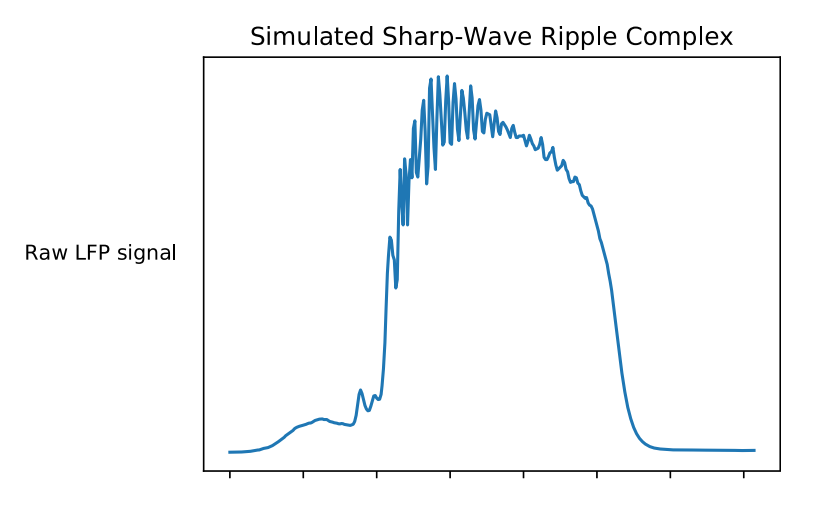
\includegraphics[width=0.75\linewidth]{images/Sharp Wave Ripple Complex.png}
        \caption{Plot of a raw LFP trace \cite{Aussel.2018}}
        \label{fig:sharp-Wave-Ripple}
    \end{figure}


    \subsection{Automated Sharp Wave Ripple Detection}
    
    The occurrence and properties of sharp wave ripples are the most important aspects of the output for this thesis. Their automatic identification and analysis are therefore essential, to allow for an efficient evaluation of different brain states. Unfortunately, a common standard for this procedure, which comes with several methodological challenges, is nonexistent \cite{Liu.2022}. As a consequence, the analysis of this work is in large parts based on the approach presented by \textcite{AmelieAussel.2020}, that already was used with the model. However, a few thresholds and procedures had to be adjusted to accommodate the employed model configuration and use case.\\
    The resulting detection algorithm can be divided into two stages. The \textit{detection of the sharp wave}, followed by the \textit{frequency analysis}, which analyzes candidate waves (also called events) for a superimposed ripple.
    
    % Detecting sharp wave
        % with help of rms standard deviation
            % unusual strong signal
            % exeeding a threshold that can be defined
                % is parameter that needs to be configured
                % mention specific values used
    To detect the large amplitude deflection of a \textbf{sharp wave}, the signal's root mean square (RMS) is calculated, based on non-overlapping time windows of 10ms. These RMS values are a reference for the signal power \cite{glaser.2012}. Then their standard deviation (SD) is extracted, which can be used to identify unusually strong signal portions. For a signal portion to be considered a sharp wave, its RMS values must be larger than 3 times the SD, reaching a peak of at least 4.5 times the SD.\\ 
    % checking if the strongest frequency in sharp wave is ripple
        % extracting spectral density
            % which frequency has how much power
        % range of qualifying peak frequncy is parameter
            % was chosen to be ...
    The sharp waves identified like this, then need to be \textbf{analyzed in} terms of their \textbf{power spectrum}. This is performed by first bandpass filtering the signal parts between 30 and 400Hz (employing a Butterworth filter of second order) and therefore discarding especially the lower frequencies of high power. Followed by the extraction of the frequency of the highest power in the remaining range. This \textit{peak frequency} is the most relevant oscillation pattern imposed on the sharp wave and defines, whether it qualifies as a ripple or not. For this work, the frequency range, supposed by \textcite{vanQuyen.2010} was used, defining every sharp wave with a superimposed peak frequency between 100-250Hz, as a sharp wave ripple (complex).
    

 
\section{Electromagnetic Attacks}
% general elaborations on attack design
% Because no specific proposal for the simulation of such an attack exists
    % Exploring different mechanisms that could lead to the observed symptoms
        % first evaluate the relevance of each aspect
        % propose and evaluate possible combinations that could represent a full attack
% (as foundations showed) different categories of mechanisms exist
    % specifically Neurotransmitter changes, Structural damage and alterations of input identified as promising and will be explored
    As discussed in the previous chapter, the topic of Neurostrikes is very novel, and their inner mechanisms are not fully understood. As a consequence, also no specific proposals on the integration of such an attack in a brain simulation exist. Therefore, this work explores potential underlying mechanisms that could be responsible for the symptoms associated with Neurostrikes. Focusing primarily on the reported memory and learning impairments, to establish a basis for further research and the development of countermeasures.\\
    Different mechanism categories have been identified, that could be involved in such impairments. Specifically \textit{changes in neurotransmitters} and \textit{structural damage} to the hippocampus showed promising connections to both electromagnetic radiation and memory performance. How each of these categories was designed, will be presented below. Followed by the discussion and proposal of combinations of them, resulting in full-scale attacks. 


    \subsection{Neurotransmitter Changes}
    % As hu showed, influence of rf emr on neurotransmitters well documented
        % has to be stated that the results are not uniform
        % might be caused by large radiation parameter variability between experiments
    % Changes in acetylcholine seem to have an impact on memory consolidation Hu.2021, Aussel.2018
    % papers like Fujiwara.1978, Hu.2021  idnetified an increase of it
        % specifically 1.2x - 2.5x (Fujiwara.1978)
    % since Aussel also investigated ACh levels in model, integration easy
        % adjustment of parameter values (gCAN and G_ACh)
            % mention their impact
        % realistic value range based on observed level change
            % top level metioning of literature and resulting range
    
    As \textcite{Hu.2021} showed, RF EMR can have an impact on many neurotransmitter levels in the brain. However, the specific results of different studies are not uniform, which the authors attribute to the large variance in parameters and conditions of the experiments.\\
    Especially the neurotransmitter acetylcholine is of interest for this work, as it is affected by RF EMR \cite{Hu.2021} \cite{Fujiwara.1978}, and is associated with memory processes \cite{Aussel.2018}. Specifically, an increase in this neurotransmitter has been reported \cite{Hu.2021}, which as \textcite{Fujiwara.1978} found can manifest in up to 2.5 times the concentration, compared to the standard values of the waking state.\\
    The integration of such changes into the simulation is already supported by the model, as the acetylcholine levels were already a parameter of interest for the model creators \cite{Aussel.2018}. They investigated the varying concentrations across the sleep-wake cycle and realized their effect with the help of the parameters \textit{gCAN} and \textit{gACh} \cite{HippSimModel.2}. Whilst \textit{gCAN} represents the conductance of a "Calcium-Activated-Nonspecific" (CAN) ion channel \cite{Aussel.2018}, \textit{gACh} defines a factor that influences a series of synaptic conductances inside sub-regions of the hippocampus. More specifically, it increases both the excitatory synaptic conductances inside the DG, as well as the inhibitory synaptic conductances in the DG and CA1 region. Conclusively, \textit{gACh} also decreases the excitatory synaptic conductances inside the EC and CA3 region \cite{AmelieAussel.2020}.\\
    In the context of their work, \textcite{Aussel.2018} defined two values for each of the parameters, representing the sleep or waking state respectively (\(gCAN : [0.5\mu S/cm^2, 25\mu S/cm^2]\), \(gACh : [1, 3]\)). These values need to be associated with a concentration of acetylcholine, to be able to define realistic values for the simulation of an attack. Due to a lack of comparable absolute values, this was done with relative observations. \textcite{Hasselmo.1999} states that the neurotransmitter level during sleep is about a third of the one during the waking state. Combined with the findings of \textcite{Fujiwara.1978} (documenting an increase due to radiation of up to 2.5 times relative to waking concentrations), this work concluded that an attack during the sleeping state, could result in similar levels as the ones during waking state (\(gCAN = 25\mu S/cm^2\), \(gACh = 3\)). However, since these estimations are based on observations, of which the comparability, robustness, and precision are very limited, a range of values was explored nonetheless to allow for more meaningful evaluations. The waking values constituted thereby the strongest deviation of the sleeping values and upper bound of the explored range.
    

    \subsection{Structural Damage}
    % result from rf emr
    % influence learning and memory
    % specific magnitude of changes
    % how integrated
    Different forms of structural damage have been observed as a consequence of electromagnetic radiation \cite{Shahin.2015} \cite{Tan.2017}. Due to the employed model, those affecting the hippocampus are of particular interest for this work. Also because damages affecting this brain area, are considered as a potential cause of memory and learning impairments \cite{Narayanan.2019}. Specific observations reported \textit{damage to neurons} \cite{Shahin.2015} \cite{Altun.2017}, but also \textit{damage to synapses} \cite{Tan.2017} \cite{Xu.2006}.
    
    Concerning affected \textbf{neurons}, \textcite{Shahin.2015} reported an increase in both neuronal but also non-neuronal cell deaths, following the exposure to 2.45GHz (RF \cite{BORTKIEWICZ.2019}) radiation. These findings were supported by the observations of \textcite{Altun.2017}, who further quantified the observed neuron reduction in the whole hippocampus to be 40\%. Although, it has to be stated that this reduction was measured after long-term exposure (1 hour every day for 15 days).\\
    Integrating such a reduction of neurons into the simulation is also already facilitated by a parameter of the model (\textit{N}). It defines the maximum amount of the largest excitatory neuron groups and scales the others proportional to this value \cite{HippSimModel.2}. Its standard value is 10'000, resulting in the amounts displayed in table \ref{tab:population_sizes}. For example, a 10\% reduction to 9'000 would also result in a 10\% reduction of all the other values. To also asses less severe states like the one documented by \textcite{Altun.2017}, the whole range from 6'000-10'000 neurons will be explored. 

    \begin{table}[h]
        \centering
            \begin{tabular}{@{}lcc@{}}
                \toprule
                Region & $N_E$ & $N_I$ \\ 
                \midrule
                Entorhinal cortex & 10'000 & 1'000 \\
                Dentate Gyrus & 10'000 & 100 \\
                CA3 & 1'000 & 100 \\
                CA1 & 10'000 & 1'000 \\ 
                \bottomrule
            \end{tabular}
        \caption{Number of excitatory neurons (\(N_E\)) and interneurons (\(N_I\)) in each region \cite{Aussel.2018}}
        \label{tab:population_sizes}
    \end{table}
    

    Damage to \textbf{synapses} in the hippocampus was characterized by \textcite{Xu.2006}, stating that 1.8GHz radiation, might lead to reduced synaptic activity and synapses in general. However, more specific findings were the amplitude reductions of excitatory postsynaptic currents. This finding was also quantified and amounted to a reduction of 20\%.\\
    To integrate this effect into the simulation, the model parameter \(g\_max\_e\) is perfectly suited, as it defines the maximum conductance of all excitatory synapses. Since its standard value is defined as \(60pS\), a 20\% reduction would amount to \(48pS\) which represents the lower bound of the explored value range for this parameter. 


    %\subsection{Input Alterations}
    %Since the impact of radiofrequency electromagnetic radiation is not restricted to the hippocampus \cite{Lai.1994}, the stimuli reaching the structure most likely are altered as well. These alterations, would for example reflect a decrease of spontaneous activity as documented by \textcite{seaman1978slow} and \textcite{wachtel1975effects}.\\
    %To integrate such a reduced activity, different parameters of the input can be adjusted. For example, the measurement amplitude or frequency to which the measurements are scaled could be reduced. Exact values are in this context difficult to specify theoretically, which is why also for this type of mechanism, a range of values in these parameters will be explored.

    \subsection{Full Attack}
    To represent a full-scale attack, these mechanisms and adjusted parameters can simply be combined to different extents. This enables a type of worst-case scenario, where all parameters are applied at their extreme values, but especially the exploration of a more realistic brain state under attack, as these mechanisms will most likely not be triggered selectively.\\
    Guided by the relation between radiation intensity and its effect on the brain, the \textit{Full Attack} will be explored with parameter combinations, that could arise from the same level of radiation exposure. This was achieved by defining 4 different intensity steps across the value range of every parameter, where the highest value represents the strongest deviation from the healthy sleep values in the range. Values of the same intensity level were then combined, to simulate different levels of overall radiation intensity. 


%\section{Countermeasure}
